\documentclass[a4paper,12pt]{jarticle}
\usepackage[dvipdfmx]{graphicx}
\usepackage{amsmath}
\usepackage{subfigure}
\usepackage{comment}

\setlength{\hoffset}{0cm}
\setlength{\oddsidemargin}{-3mm}
\setlength{\evensidemargin}{-3cm}
\setlength{\marginparsep}{0cm}
\setlength{\marginparwidth}{0cm}
\setlength{\textheight}{24.7cm}
\setlength{\textwidth}{17cm}
\setlength{\topmargin}{-45pt}

\renewcommand{\baselinestretch}{1.6}
\renewcommand{\floatpagefraction}{1}
\renewcommand{\topfraction}{1}
\renewcommand{\bottomfraction}{1}
\renewcommand{\textfraction}{0}
\renewcommand{\labelenumi}{(\arabic{enumi})}
%\renewcommand{\figurename}{Fig.} %図をFig.にする


%図のキャプションからコロン:を消す
\makeatletter
\long\def\@makecaption#1#2{% #1=図表番号、#2=キャプション本文
\sbox\@tempboxa{#1. #2}
\ifdim \wd\@tempboxa >\hsize
#1 #2\par 
\else
\hb@xt@\hsize{\hfil\box\@tempboxa\hfil}
\fi}
\makeatother
% 


\title{電機システム制御特論 \\
Assignment (2016/05/20)\\
}
\author{\vspace{40mm}\\
九州工業大学大学院 \hspace{0mm} 工学府\\
機械知能工学専攻\ \hspace{0mm} 知能制御工学コース \\
\vspace{5mm}\\
所属:\ 西田研究室\\
学籍番号:\ 16344217\\
提出者氏名:\ 津上 \hspace{0mm} 祐典\\\vspace{5mm}\\ }
\date{平成28年\ 5月\ 27日}

\begin{document}

%表紙
\titlepage
\maketitle
\thispagestyle{empty}

\newpage

\thispagestyle{empty}
\tableofcontents

\newpage
\setcounter{page}{1}
%%%%%%%%%%%%%%%%%%%%%%%%
\section{問題}
%%%%%%%%%%%%%%%%%%%%%%%%
Consider the following system
%
\begin{eqnarray}
 \begin{cases}
  x = ax + bu + v & \\
  y = x + w
 \end{cases}
\end{eqnarray}
%

where $a=-0.02$ , $b=0.001351$, and $v$ and $w$ are both White Gaussian
noise $E \bigl\{ v^2 \bigr\} = E \bigl\{ w^2 \bigr\} = 0.7$.
Design kalman filter for the system, and demonstrate the performance
with computer simulations.

%%%%%%%%%%%%%%%%%%%%%%%%
\section{カルマンフィルタとは}
%%%%%%%%%%%%%%%%%%%%%%%%
カルマンフィルタとは,雑音が入った観測値を用いて,ある動的システムの状
態推定(フィルタリング)するものである.状態方程式の状態推定する方法
として,ルーエンバーガによるオブザーバ(状態推定器)が有名であるが,これ
は雑音などが存在しない確定的な場合を対象としている.それに対して,カルマ
ンフィルタは,確定的な枠組みで状態推定問題を検討した.カルマンフィルタで
は,雑音の正規白色性を仮定することにより,システマティックに最適設計が可
能という優位点を持つ.制御対象の正確なモデルを利用できれば,状態推定
(フィルタリング)することが出来る.これは,カルマンフィルタの重要なポイ
ントである.つまり,制御対象のモデリングの正確さがカルマンフィルタの精度
に関わってくる.図\ref{fig:kalman_m}に,あるシステムにカルマンフィルタを適
応したものを示す.図\ref{fig:kalman_m}に示す一入力一出力のシステム
\begin{eqnarray}
 \begin{cases}
  \dot{x}=Ax+bu+v & \\
  y = cx + w
  \end{cases}
\end{eqnarray}
を考える.ここで$(A,c)$の組は可観測である.また,$v$はシステムノイズであ
り,$w$は観測ノイズである.これらの2つのノイズは白色ガウシアンノイズと
呼ばれており,
\begin{eqnarray}
 \begin{cases}
  E \bigl\{v(t)\bigr\} = 0 \ , \ E \bigl\{w(t)\bigr\} = 0 & \\
  E \bigl\{v(t)v(\tau)^T\bigr\} = Q\delta (t - \tau) \ , \  E
  \bigl\{w(t)w(\tau)^T\bigr\} = r\delta (t - \tau) & \\
  E \bigl\{v(t)w(\tau)\bigr\} = 0  
 \end{cases}
\end{eqnarray}
と表される.
%
\begin{figure}[tbp]
 \begin{center}
  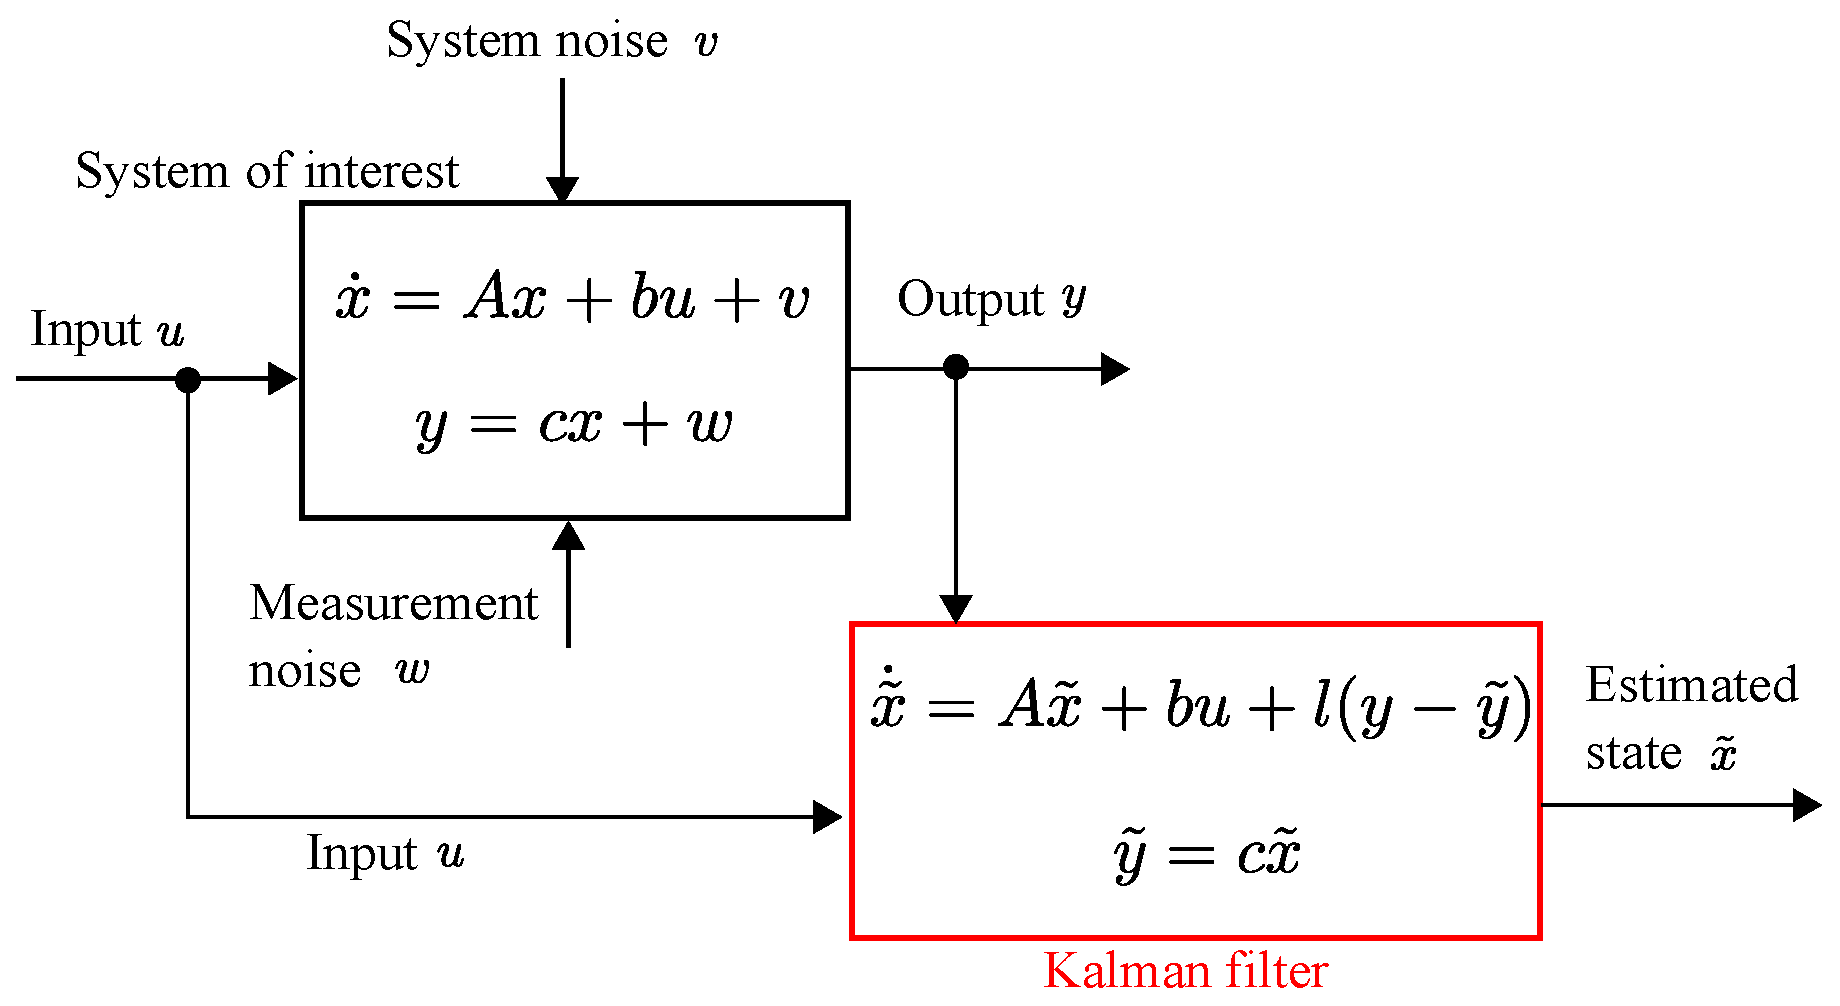
\includegraphics[width = 150mm]{fig/kalman_model.eps}
 \end{center}
 \caption{カルマンフィルタ}
 \label{fig:kalman_m}
\end{figure}
%
%%%%%%%%%%%%%%%%%%%%%%%%
\section{カルマンフィルタの設計}
%%%%%%%%%%%%%%%%%%%%%%%%
カルマンフィルタを設計するために,カルマンゲイン$l$を導出する.カルマ
ンゲインは以下の式より導出できる.
\begin{equation}\label{equ:gain}
 l = \frac{1}{r}Pc^T
\end{equation}
ただし,$P$はリッカチ方程式
\begin{equation}\label{equ:ricca}
 AP + PA^T -\frac{1}{r}Pc^TcP = -Q 
\end{equation}
の実正定行列解である.(\ref{equ:ricca})式に
\begin{eqnarray}
 \begin{cases}
  A = -0.02 & \\
  r = 0.7 & \\
  Q = 0.7 & \\
  c = 1
 \end{cases}
\end{eqnarray}
を代入し,整理すると
\begin{equation}
 P^2 + 0.028P -0.49 = 0
\end{equation}
を得る.$P > 0$より上式の解は
\begin{equation}
 P = 0.686
\end{equation}
となる.するとカルマンゲイン$l$は,
\begin{equation}
 l = \frac{1}{0.7} \times 0.686 \times 1 = 0.98
\end{equation}
となる.したがってカルマンフィルタは以下の式で与えられる.
\begin{eqnarray}
 \begin{cases}
\dot{\tilde{x}} = -0.02x + 0.001351u + 0.98 \big(y - \tilde{y} \big)
  & \\
  \tilde{y} = \tilde{x}
 \end{cases}
\end{eqnarray}


%%%%%%%%%%%%%%%%%%%%%%%%
\section{シミュレーション}
%%%%%%%%%%%%%%%%%%%%%%%%
制御入力(ステップ入力)$u$を$u=1000$としてMATLAB/Simulinkでシミュレーションを行った.こ
のとき,構成したSimulinkのモデルを図\ref{fig:kalman_b}に示す.また,シミュ
レーション結果を図\ref{fig:kalman_g}に示す.また,Timeが300から400のとき
の拡大図も図\ref{fig:kalman_g}に合わせて示す.ただし,システムノイズ$v$を
$v=0$とし,シミュレーションを行った.
%
\begin{figure}[bp]
 \begin{center}
  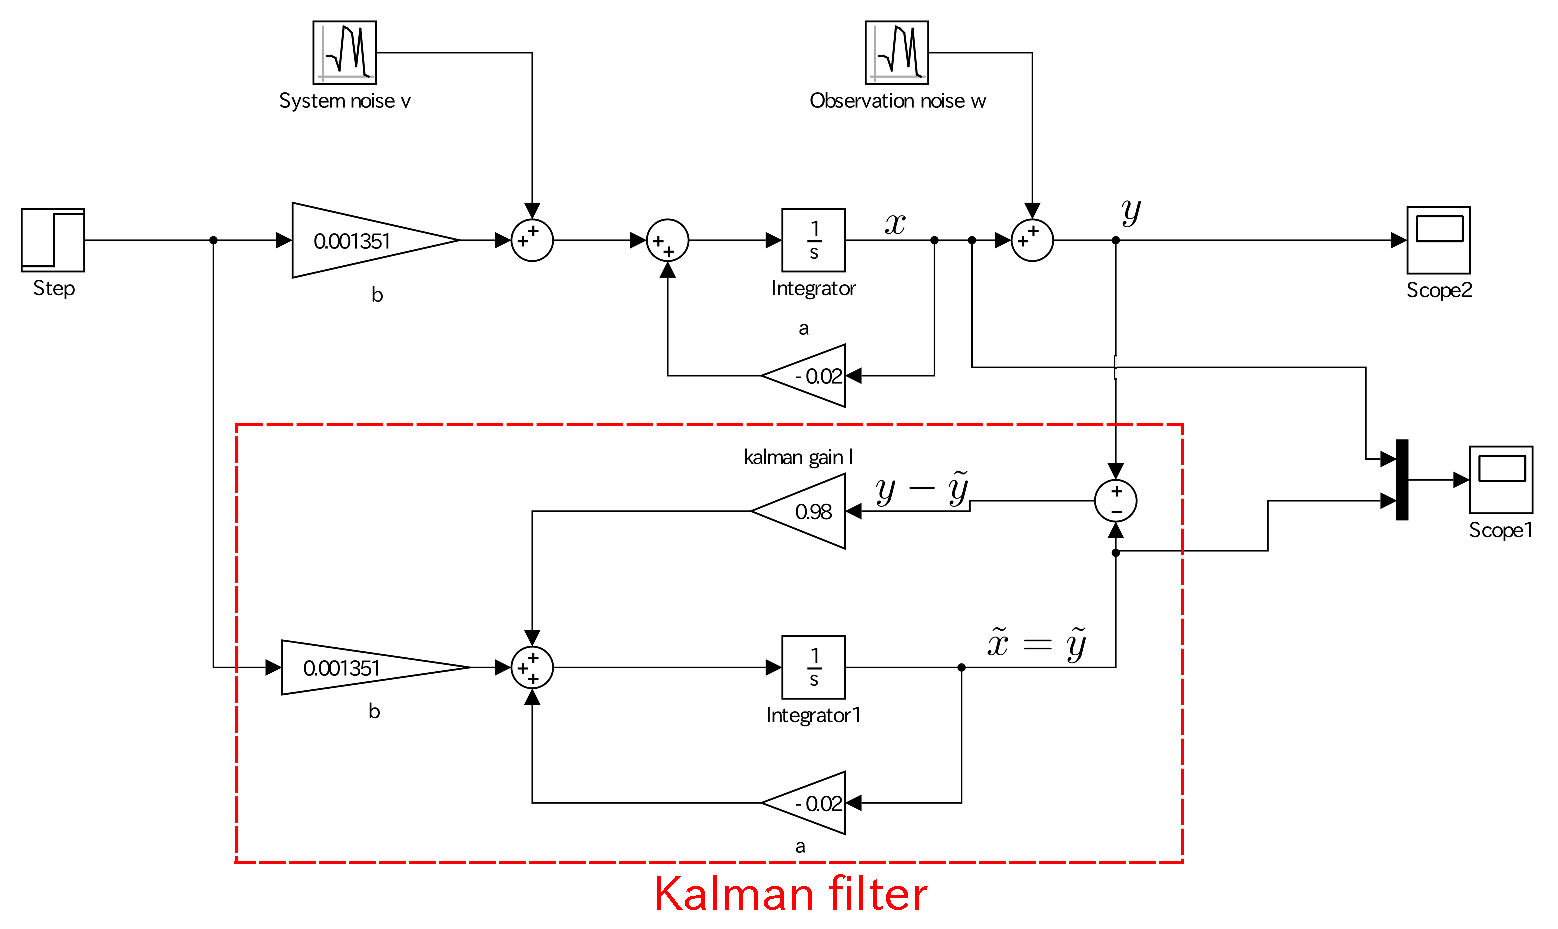
\includegraphics[width = 150mm]{fig/kalmanfilter2.eps}
 \end{center}
 \caption{simulinkで構成したモデル}
 \label{fig:kalman_b}
\end{figure}
%
\begin{figure}[htbp]
 \begin{center}
  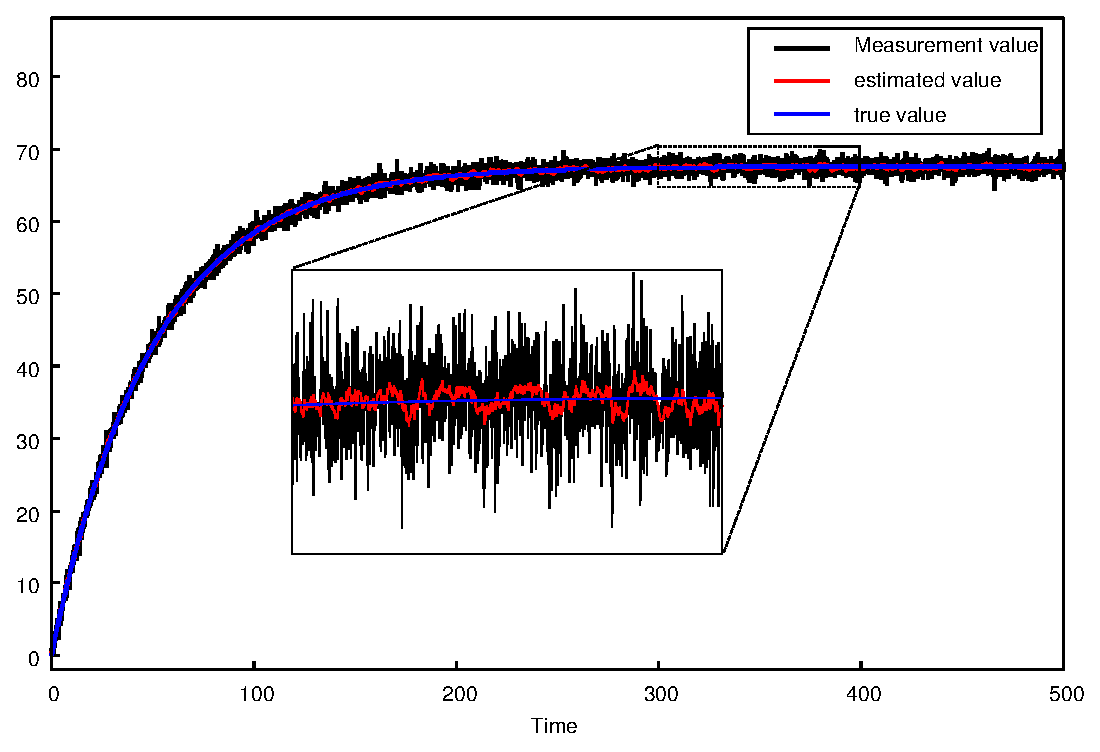
\includegraphics[width = 170mm]{fig/kalmanfilterG2.eps}
 \end{center}
 \caption{シミュレーション結果}
 \label{fig:kalman_g}
\end{figure}
%
\newpage
%%%%%%%%%%%%%%%%%%%%%%%%
\section{考察}
%%%%%%%%%%%%%%%%%%%%%%%%
図\ref{fig:kalman_g}を見ると,カルマンフィ
ルタを用いた推定値($\tilde{y}=\tilde{x}$)が測定値($y=x+w$)より観測ノ
イズを除いた真値($y=x$)との誤差が小さいことがわかる.つまり,カルマンフィ
ルタを使ったことにより観測ノイズの影響を抑えていることがわかる.本レポー
トでは,システムノイズや観測ノイズの分散が既知としてシミュレーションを行っ
たが,現実世界ではノイズの正確な分散を得るのは難しい.よって,カルマンゲ
イン$l$を一定にするのでなく,ノイズの変化に合わせて$l$も変化させなければ
ならないと考えられる.また,節で述べたように制御対象のモデル化の精度にも
状態推定の精度が関わってくるため,制御対象をモデル化も精度良く行わなけれ
ばならないと考えられる.
%
\begin{thebibliography}{99}
\addcontentsline{toc}{section}{参考文献}

 \bibitem{denki} T.Sakamoto,
		 "Lecture Notes of Advanced Electrical Drive Control System", 2016.

 \bibitem{adachi} 足立修一,丸田一郎,"カルマンフィルタの基礎",東京電機
		 大学出版局,2014.

\end{thebibliography}

\end{document}
